\documentclass[10pt,a4paper]{article}

\usepackage[T1]{fontenc}
\usepackage[utf8]{inputenc}
\usepackage{lmodern}
\usepackage[margin=2.3cm]{geometry}
\usepackage{amsmath}
\usepackage{graphicx}
\usepackage{booktabs}
\usepackage{multicol}
\usepackage{xcolor}
\usepackage{listings}
\usepackage[colorlinks=true,linkcolor=blue!55!black,urlcolor=blue!55!black,citecolor=blue!55!black,pdftitle={Moving Like a Human}]{hyperref}

% ---------------------------------------------------------------- listings --
\definecolor{kw}{RGB}{21,82,154}
\definecolor{cm}{RGB}{20,110,40}
\definecolor{st}{RGB}{175,95,20}

\lstdefinestyle{code}{
  language=Python,
  basicstyle=\ttfamily\scriptsize,
  keywordstyle=\color{kw}\bfseries,
  commentstyle=\color{cm}\itshape,
  stringstyle=\color{st},
  showstringspaces=false,
  columns=fullflexible,
  keepspaces=true,
  breaklines=true,
  frame=single,
  rulecolor=\color{gray!45},
  framerule=0.4pt,
  backgroundcolor=\color{gray!7},
  xleftmargin=6pt,
  framexleftmargin=4pt,
  captionpos=b,
  aboveskip=6pt,
  belowskip=6pt,
}

\lstdefinestyle{shell}{
  basicstyle=\ttfamily\footnotesize,
  columns=fullflexible,
  keepspaces=true,
  breaklines=true,
  frame=single,
  rulecolor=\color{gray!45},
  framerule=0.4pt,
  backgroundcolor=\color{gray!7},
  captionpos=b,
  aboveskip=6pt,
  belowskip=6pt,
}

\newcommand{\code}[1]{\texttt{#1}}
\newcommand{\loss}{\ensuremath{\mathcal{L}}}

% tighter float packing (the document is float-heavy: listings, tables, figure)
\renewcommand{\topfraction}{0.92}
\renewcommand{\bottomfraction}{0.8}
\renewcommand{\textfraction}{0.07}
\renewcommand{\floatpagefraction}{0.85}
\setlength{\floatsep}{8pt plus 2pt minus 2pt}
\setlength{\textfloatsep}{10pt plus 2pt minus 4pt}
\setlength{\intextsep}{10pt plus 2pt minus 4pt}

\title{\textbf{Moving Like a Human}\\[2mm]
\large An Elo-Conditioned Transformer for Predicting Human Chess Moves}
\author{} % add your name here
\date{October 19, 2026}

\begin{document}
\maketitle

\begin{abstract}
\noindent
This paper documents \emph{chess3}, a complete, end-to-end system that learns
to predict the chess moves a \emph{human} player would make, conditioned on
that player's Elo rating. Given the rating, the current position, and the
last five moves, a 26.4-million-parameter transformer outputs a probability
distribution over the legal moves in the position. The system was trained on
119\,million individual move decisions extracted from 1.8\,million games of
the open Lichess database. We describe the full pipeline: how two million
games become 132\,million fixed-size binary training records, how a position
is tokenized into a fixed 74-token sequence with one embedding table per
field, why the loss function restricts the softmax to the \emph{legal} moves
of each position, how training remains resumable across archives of fresh
data, and how three evaluation reports measure not only prediction accuracy
but also \emph{Elo fidelity} --- whether the model actually behaves
differently at different ratings. At the time of writing the model reaches a
held-out cross-entropy of 1.69 nats (perplexity $\approx$ 5.4 effective move
choices) on its first data chunk, against 3.39 nats for uniform guessing
among the $\sim$30 legal moves of a typical position. The paper is written
for readers \emph{new to machine learning}: every design decision is
explained from first principles, alongside the exact code that implements it.
\end{abstract}

\setcounter{tocdepth}{1}
\tableofcontents

% =====================================================================
\section{Introduction}\label{sec:intro}

Chess engines are superhuman. Stockfish and its neural descendants evaluate
positions with a precision no human can match, and a modern engine playing
at full strength is simply not fun to play against for a club player. But
there is a different, less explored problem: instead of asking
\emph{``what is the best move here?''}, ask \emph{``what would a human of
rating 1400 do here?''}. That question has practical answers --- it would
let us build training opponents that feel human, study how skill expresses
itself in move choice, and generate believable move distributions for any
strength level.

This project, \emph{chess3}, answers the human question with supervised
deep learning. The contract of the system is:

\begin{quote}
\textbf{Input:} the Elo rating of the player to move, the current position,
and the last five moves (in PGN form).\\
\textbf{Output:} a probability for every \emph{legal} move in the position,
e.g.\ $[\,\texttt{e5}: 0.42,\ \texttt{Nf6}: 0.31,\ \dots\,]$.
\end{quote}

Two properties make this more than a toy. First, the model is
\emph{conditioned on Elo}: the same position yields a different move
distribution for a 1000-rated and a 2000-rated player, so one model
covers a whole spectrum of strengths. Second, the model emits a
\emph{distribution}, not a single move --- human play is not
deterministic, and sampling from the distribution reproduces the
variety of human choice. Conceptually, the task is next-token
prediction, the workhorse of language models~\cite{gpt2}, transplanted
to chess: a move decision becomes a supervised example, the position
plus recent history is the ``context,'' and the move is the ``token''
to predict. Three chess-specific twists make the transplant interesting:
the action space is \emph{variable} (each position has its own set of
legal moves, about 30 on average), the conditioning signal (Elo) must
actually influence the output for the model to be useful, and the data
is enormous --- every ply of every game is one sample.

\paragraph{System map.} The repository is a pipeline of small scripts, each
with one job; the paper follows this order.

\begin{table}[htbp]
\centering
\small
\begin{tabular}{@{}ll@{}}
\toprule
\textbf{Script} & \textbf{Role} \\
\midrule
\verb|download_lichess_db.py| & fetch a monthly Lichess archive (resumable \code{.pgn.zst}) \\
\verb|process_lichess_db.py| & games $\rightarrow$ binary train/eval shards + legal-move lists \\
\verb|move_vocab.py| & generate \code{moves.json}: the 1{,}968-move vocabulary \\
\verb|train.py| & train the transformer; write checkpoints + loss history \\
\verb|plot_loss.py| & render \verb|loss_history.jsonl| into a loss curve \\
\verb|evaluate.py| & move-match, cross-Elo matrix, and KL probes \\
\verb|infer.py| & one position $\rightarrow$ JSON move probabilities \\
\verb|gui/| & React board + controls; calls \code{infer.py} per move \\
\bottomrule
\end{tabular}
\caption{The system at a glance. Section~\ref{sec:data} covers the first
three rows, Sections~\ref{sec:arch}--\ref{sec:train} the model and its
training, Section~\ref{sec:eval} evaluation, Section~\ref{sec:infer}
inference and the GUI.}
\label{tab:map}
\end{table}

\paragraph{How to read this paper.} Section~\ref{sec:primer} is a compact
primer defining every machine-learning term used later, each with a chess
example attached; skip it if you know the basics. From
Section~\ref{sec:data} on, every design decision is presented together
with the actual code that implements it, lightly trimmed for space ---
trimmed spots are marked with \code{\# ...} comments.
Section~\ref{sec:results} reports the real training numbers from the
project's checkpoints, and Section~\ref{sec:limits} discusses what the
system cannot do.

% =====================================================================
\section{A Primer for the Machine-Learning Beginner}\label{sec:primer}

This section defines the vocabulary used in the rest of the paper. Each
concept appears exactly where the project uses it, so the definitions can
be checked against real code later.

\paragraph{Supervised learning.} We are given many pairs $(x_i, y_i)$ ---
an \emph{input} and the \emph{correct output} --- and want a model that,
given a new $x$, produces a probability distribution $p(y \mid x)$ over
outputs. Here $x_i$ is ``position + Elo + last five moves'' and $y_i$ is
the move a human actually played. The examples come from data (1.8M real
games), so the model \emph{imitates} humans rather than being told any
chess rule.

\paragraph{Tokens.} A \emph{token} is a categorical value converted to an
integer id. Chess positions are not text, so we design the tokenization
ourselves: a position is 64 square tokens (one per board square), plus
one Elo token, one side-to-move token, and so on --- 74 tokens in total
(Section~\ref{sec:tokenization}). A \emph{vocabulary} is the fixed list
of possible values a token can take; e.g.\ a square token takes one of 13
values (empty, or one of the 12 piece/color combinations).

\paragraph{Embeddings.} An \emph{embedding} turns an integer id into a
vector of learned numbers: a lookup table with one row per vocabulary
entry, here 512 numbers per row. Row $k$ \emph{is} the model's learned
representation of value $k$, and the rows are trained like any other
parameter. Ids are arbitrary --- id 7 and id 8 (say, the white and black
bishop) are not ``close'' unless training makes them so.

\paragraph{Logits and softmax.} The model's last layer produces a raw
score, a \emph{logit}, for every possible output (here: every move id). To
turn scores into a probability distribution we apply the
\emph{softmax}:
\begin{equation}
p_i \;=\; \frac{e^{z_i}}{\sum_j e^{z_j}},
\label{eq:softmax}
\end{equation}
where $z_i$ is the logit of move $i$. Big logits get big probabilities;
the \emph{temperature} $T$ divides the logits first
($z_i/T$) --- a higher $T$ flattens the distribution (more variety), a
lower $T$ sharpens it toward the single best move.

\paragraph{Cross-entropy and perplexity.} The quality of a probability
prediction is measured by the \emph{cross-entropy} of the outcome that
actually happened:
\begin{equation}
\loss \;=\; -\log p(y_{\text{true}}).
\label{eq:ce}
\end{equation}
If the model put probability 1 on the human's move, $\loss = 0$; if it put
probability $p$, the loss is $-\log p$. Training \emph{is} minimizing the
average of this quantity over millions of examples. A useful reading aid:
$e^{\loss}$ (the \emph{perplexity}) is ``how many equally-likely options
the model was effectively choosing among.'' A loss of $\ln 5 \approx 1.61$
means, roughly, the model behaved as if the human's move was drawn
uniformly from 5 candidates. Compare that with the $\sim$30 legal moves of
a typical position: uniform guessing among them would cost
$\ln 29.7 \approx 3.39$.

\paragraph{Attention and transformers.} A \emph{transformer}
block~\cite{attention} updates each token's vector by letting it gather
information from the other tokens. In \emph{attention}, every token emits a
query, a key and a value (three learned projections of its vector); token
$a$'s new content is a weighted average of all tokens' values, where the
weight of token $b$ is the softmax of the dot product $q_a \cdot k_b$ ---
``how relevant is $b$ to understanding $a$?'' A \emph{head} is one such
pattern learned in a subspace (this model has 8 heads of 64 dimensions
each, applied in parallel). Because attention has no notion of order, a
learned \emph{positional embedding} is added to each token so slot 5 and
slot 50 can be distinguished. Language models usually restrict attention
to look only \emph{leftward} (they generate the next token); here the
whole position is known at once, so attention is unrestricted --- but the
sequence itself is never the target of a prediction; the target is an
external move id (Section~\ref{sec:arch} explains where the answer is read
out).

\paragraph{Optimization.} Training adjusts parameters to reduce the loss,
one small \emph{batch} of examples (here 512) at a time. The
\emph{optimizer} computes, for each parameter, a step direction and size.
\emph{AdamW}~\cite{adamw} keeps a running average of each parameter's
gradient and of its squared gradient, and scales the step per parameter
accordingly; \emph{weight decay} additionally shrinks weights a little
every step, which fights overfitting. The \emph{learning rate} is the
global step size --- too large and training oscillates, too small and it
crawls; real runs change it over time with a \emph{schedule}. One full
pass over the training data is an \emph{epoch} --- here one epoch is 119M
samples, i.e.\ about 233k optimizer steps of batch 512.

\paragraph{Overfitting and held-out data.} A model can memorize its
training examples instead of learning the underlying regularity. To
detect this, a slice of the data is held out (here 10\% of the
\emph{games}) and never trained on; the \emph{eval loss} on that slice
estimates performance on unseen positions. Train loss improving while
eval loss stagnates is the memorization signal.

% =====================================================================
\section{Data: From Two Million Games to 132 Million Samples}\label{sec:data}

\subsection{Source and download}

The data is the Lichess open database~\cite{lichess}: one freely
downloadable archive per month of every \emph{standard, rated} game played
on the server --- roughly two million games and $\sim$1.5\,GB compressed
per month. \verb|download_lichess_db.py| fetches one month
(\code{--month 2026-05}) with resume support and progress reporting, and
stores it in \code{data/} as a \code{.pgn.zst} archive named after the
month.

The archive is PGN text (the standard game-notation format) compressed
with zstandard. Each game carries headers with both players' ratings ---
and rating is precisely the conditioning signal we need, so games whose
headers lack an Elo are discarded during processing.

\subsection{One sample per move decision}

The unit of training is not a game but a \emph{move decision}. Walking
through a game ply by ply, each position ``before the move'' becomes an
input, and the move the player chose becomes the target. Listing~\ref{lst:records}
shows the constructor; it also precomputes, for every position, the id
list of the \emph{legal} moves (used by the loss in
Section~\ref{sec:train}).

\begin{lstlisting}[style=code, caption={One (record, legal-id-list) pair per
mainline move of a game (\code{process\_lichess\_db.py}). The
\code{deque} with \code{maxlen=5} is a sliding window: initialized to five
pad tokens, it forgets the oldest move every time a new one is appended.},
label={lst:records}, float=htbp]
def promo_char(move):
    return "" if move.promotion is None else chess.piece_symbol(move.promotion)

def create_game_records(game, white_elo, black_elo, move_to_id):
    """One (record, legal_ids) pair per mainline move of a game."""
    board = game.board()
    history = deque([NONE_MOVE] * HISTORY_SIZE, maxlen=HISTORY_SIZE)
    records = []

    for move in game.mainline_moves():
        squares, stm, castling, ep = board_to_fields(board)
        target = move_to_id[(move.from_square, move.to_square, promo_char(move))]
        legal = [
            move_to_id[(legal.from_square, legal.to_square, promo_char(legal))]
            for legal in board.legal_moves
        ]
        player_elo = white_elo if board.turn == chess.WHITE else black_elo
        records.append(
            ((tuple(squares), player_elo, stm, castling, ep, target, tuple(history)), legal)
        )
        board.push(move)
        history.append(target)

    return records
\end{lstlisting}

Three details matter. The Elo stored with each sample is the rating of
the \emph{player to move} in that position, not a single game-level
value --- within one game, White's and Black's decisions get their own
conditioning. The history is the \emph{UCI ids} of the last five moves
(Section~\ref{sec:tokenization}), front-padded with the special
\code{NONE\_MOVE} id when the game has fewer than five moves, so every
sample always has exactly five history tokens.

Games with missing Elo or PGN errors are skipped (in the processed chunk
used in this paper: zero games skipped). The 1.8M games yield
119{,}096{,}505 training and 13{,}157{,}576 evaluation samples --- on
average 66 move decisions per game, one per ply.

\subsection{The 80-byte record}

Every sample is stored as a fixed-width 80-byte record
(Listing~\ref{lst:record}). Fixed-width binary is a deliberate choice at
this scale: \code{np.fromfile(path, dtype=RECORD\_DTYPE)} memory-maps the
whole shard in one call with zero parsing, whereas 132M JSON objects would
need to be decoded one by one, forever.

\begin{lstlisting}[style=code, caption={The training record and its
encoder (\code{fen\_codec.py}). A position is exactly
$64+1+1+1+1 = 68$ bytes; Elo, target and history complete the 80-byte
record.}, label={lst:record}, float=htbp]
RECORD_DTYPE = np.dtype(
    [
        ("squares", np.uint8, (64,)),   # 0 empty; 1-6 white PNBRQK; 7-12 black
        ("elo", np.uint8),              # Elo bracket / 100, index 0..40
        ("stm", np.uint8),              # side to move: 0 white, 1 black
        ("castling", np.uint8),         # bit0 K, bit1 Q, bit2 k, bit3 q
        ("ep", np.uint8),               # 0 none, else en-passant square + 1
        ("target", np.uint16),          # UCI move id of the played move
        ("history", np.uint16, (HISTORY_SIZE,)),  # last 5 move ids
    ],
    align=False,
)
assert RECORD_DTYPE.itemsize == 80, RECORD_DTYPE.itemsize

def piece_code(piece):
    if piece is None:
        return 0
    return piece.piece_type if piece.color == chess.WHITE else piece.piece_type + 6

def board_to_fields(board):
    """Position fields of a record (squares, stm, castling, ep)."""
    squares = [piece_code(board.piece_at(square)) for square in range(64)]
    castling = 0
    for mask, bit in CASTLING_BITS:            # rook squares alive = right kept
        if board.castling_rights & mask:
            castling |= bit
    ep_square = board.ep_square
    ep = 0 if ep_square is None else ep_square + 1
    return squares, (0 if board.turn == chess.WHITE else 1), castling, ep
\end{lstlisting}

Note what a record does \emph{not} contain: no clocks, no repetition
counters, no material balances. Everything the model knows about the game
is the raw occupation of 64 squares, four castling bits, the en-passant
square, the side to move, five recent moves and one Elo index. If a human
strength signal lives in those fields, the model has to find it.

\subsection{Elo bucketing}

Ratings are rounded to the nearest 100 and stored as an index $0..40$
(Elo $0..4000$). Listing~\ref{lst:elo} shows the mapping.

\begin{lstlisting}[style=code, caption={Elo to embedding index
(\code{fen\_codec.py}, validation trimmed). \code{None} means ``no token
for this value'': such games are skipped at data time, and inference
rejects the input.}, label={lst:elo}, float=htbp]
def elo_bracket(elo):
    """Round a non-negative integer Elo to the nearest 100, half up."""
    return 100 * ((elo + 50) // 100)

def elo_index(value):
    """Map an Elo value or bracket to its embedding index 0..40, or None."""
    # ... int() conversion and range validation omitted ...
    bracket = elo_bracket(int(value))
    if bracket > MAX_ELO:
        return None
    return bracket // 100
\end{lstlisting}

Why round? Exact Elo values would mostly be seen once or twice, and an
embedding row trained on a handful of examples stays noise. A 100-point
bracket pools tens of thousands of decisions per bucket, and a 1347 and a
1352 player are not meaningfully different anyway. The rounding does
sacrifice fine-grained strength control at inference --- but the GUI
simply rounds the user's requested Elo to the nearest available token.

\subsection{Precomputed legal moves}

The softmax must know which moves are legal in each position
(Section~\ref{sec:losssec}). Generating legal moves with a chess library
inside the training loop would cost more time than the model's forward
pass --- so it is done \emph{once}, at data-creation time. For every
sample, \code{create\_game\_records} stores the sorted ids of its legal
moves.

The lists have variable length (0 to 218 legal moves), so they are stored
in the classic CSR layout: one flat array of ids plus one offsets array
with $n+1$ entries, where slice \code{[off[i], off[i+1])} of the flat
array holds sample $i$'s moves. Access is one line:

\begin{lstlisting}[style=code, caption={Legal-move lookup in CSR form
(\code{train.py}). Pure NumPy slicing --- no chess library anywhere near
the training loop.}, label={lst:csr}]
def legal_lists(legal_ids, offsets, indices):
    return [legal_ids[offsets[i] : offsets[i + 1]] for i in indices]
\end{lstlisting}

The 119M training samples together have 3.53\,billion legal-move ids
(7.1\,GB as \code{uint16}); that is 29.7 legal moves per position on
average --- the number to keep in mind when judging losses later.

\subsection{The 90/10 split}

The first 90\% of valid games (in archive order) become training data, the
last 10\% evaluation data. The split is by \emph{games}, not by individual
positions, on purpose: consecutive positions from one game are near-
duplicates of each other, so a random per-position split would leak
almost-identical positions into the eval set and produce flattering,
meaningless eval scores. Keeping whole games on either side also makes the
eval set a slice of \emph{later} games from the same month --- a slightly
harder, more honest generalization test than sampling uniformly.

\begin{table}[htbp]
\centering
\small
\begin{tabular}{@{}lrr@{}}
\toprule
 & \textbf{train} & \textbf{eval} \\
\midrule
games             & 1{,}800{,}000      & 200{,}000 \\
samples           & 119{,}096{,}505    & 13{,}157{,}576 \\
legal-move ids    & 3{,}532{,}207{,}631 & 389{,}098{,}118 \\
avg.\ legal moves & 29.66              & 29.58 \\
record bytes      & 9.53\,GB           & 1.05\,GB \\
legal ids bytes   & 7.06\,GB           & 0.78\,GB \\
offsets bytes     & 476\,MB            & 52.6\,MB \\
\bottomrule
\end{tabular}
\caption{The processed data shards (from \code{data/meta.json}), the
chunk used in this paper. A game yields on average 66 move-decision
samples.}
\label{tab:dataset}
\end{table}

% =====================================================================
\section{The Move Vocabulary}\label{sec:vocab}

The model outputs one logit per move, so the set of possible moves must be
fixed once and for all. The vocabulary uses UCI notation: a move is a
from-square, a to-square and an optional promotion piece --- \code{e2e4},
\code{e7e8q}, and castling written as the king's two-square trip
\code{e1g1}. This is exactly the \code{(from, to, promo)} triple used in
the data records, so ids translate losslessly in both directions.

How many moves are legal \emph{in some position}? Not $64\times64$: a move
from $a$ to $b$ only ever occurs if the geometry is right --- sliding
lines and diagonals for rooks, bishops and queens; L-shaped or
one-square steps for knights and kings; the pawn pushes, double pushes and
diagonal captures; the four castling king-trips; and the promotions.
\verb|move_vocab.py| enumerates exactly those triples
(Listing~\ref{lst:vocab}).

\begin{lstlisting}[style=code, caption={Move vocabulary enumeration
(\code{move\_vocab.py}, excerpt --- the pawn section is omitted). The
castling king-trips must be added explicitly: \code{e1g1} is not a
one-square king step, so the geometry filters above miss it.},
label={lst:vocab}, float=htbp]
def all_move_tuples():
    """Every (from, to, promo) legal in some position."""
    moves = set()
    for frm in range(64):
        fa, fr = frm % 8, frm // 8          # file, rank of the from-square
        for to in range(64):
            if frm == to:
                continue
            ta, tr = to % 8, to // 8
            df, dr = ta - fa, tr - fr
            adf, adr = abs(df), abs(dr)
            if adf == adr or df == 0 or dr == 0:          # sliders
                moves.add((frm, to, ""))
            if (adf, adr) in ((1, 2), (2, 1)) or (adf <= 1 and adr <= 1):
                moves.add((frm, to, ""))                  # knights, kings
    moves.update([(4, 6, ""), (4, 2, ""), (60, 62, ""), (60, 58, "")])  # castling
    # ... pawn pushes, captures and promotions appended analogously ...
    return moves
\end{lstlisting}

The enumeration is deterministic (the set is sorted), and its result is
written to \code{moves.json} together with a SHA-256 fingerprint of the
canonical document. Checkpoints record that fingerprint, so a later run
can \emph{refuse} to resume if the vocabulary changed underneath it ---
a cheap guard against silent id drift.

The count is 1{,}968 moves. Id 1968 is reserved for \code{<NONE>}, the
history pad token: it is \emph{never} a legal move and \emph{never} a
training target, so the model's output layer has 1{,}969 logits but the
extra one can only ever serve as padding on the input side.

% =====================================================================
\section{Tokenization: One Position, 74 Tokens}\label{sec:tokenization}

The transformer consumes a fixed sequence of 74 tokens. Table~\ref{tab:tokens}
shows the layout: one Elo token, 64 square tokens, and one token each for
side to move, castling rights, en-passant square, then five history-move
tokens, and finally one special \code{<QUERY>} token.

\begin{table}[htbp]
\centering
\small
\begin{tabular}{@{}llrl@{}}
\toprule
\textbf{Segment} & \textbf{Values} & \textbf{Count} & \textbf{Embedding table} \\
\midrule
Elo            & index 0--40 (Elo/100)          & 1  & 41 rows \\
squares        & 0, \code{PNBRQK}, \code{pnbrqk} & 64 & 13 rows + 64 rows \\
side to move   & 0 / 1                          & 1  & 2 rows \\
castling      & 4-bit mask                     & 1  & 16 rows \\
en passant     & 0 = none, else square+1        & 1  & 65 rows \\
history        & UCI move ids, front-padded     & 5  & move table (1{,}969) \\
\code{<QUERY>} & learned readout token          & 1  & a single parameter \\
\midrule
\textbf{total} &                                & \textbf{74} & \\
\bottomrule
\end{tabular}
\caption{Input tokenization. Every field gets its \emph{own} embedding
table, so ids of different fields cannot collide. The sequence length is
the same for every position --- no packing, no masking of missing fields.}
\label{tab:tokens}
\end{table}

\paragraph{One embedding table per field.} All these values are stored as
integers, and a lazy design would feed them into one shared table. The
project did that once --- and the sharing was a real bug: in a shared
vocabulary the id for ``black'' (side to move) and the id for a black
bishop on some square could collide, i.e.\ one table row had to represent
two unrelated concepts. The fix is structural: each field gets its own
table, sized exactly for its values (Table~\ref{tab:tokens}). Two fields
with the same id number now simply never meet. The tables are small ---
41, 13, 64, 2, 16, 65 rows --- so the cost is negligible.

\paragraph{Square tokens are piece + square.} A square token carries two
facts: which piece (13 options) and which square (64 options). The model
embeds both with separate tables and \emph{adds} the two vectors, exactly
like language models add a token embedding and a positional embedding:
one vector can hold both ``what'' and ``where.''

\paragraph{Tied move embeddings.} The five history tokens and the 1{,}969
output logits use \emph{the same} table: the row for \code{e2e4} is one
learned vector, whether the move appears in the input history or is being
scored as a candidate output. This is weight tying, the same trick GPT-2
uses between its input and output embeddings~\cite{gpt2} --- and here it
is even more natural than in language, because ``\code{e2e4} happened''
and ``\code{e2e4} is a candidate'' are literally the same concept.

\paragraph{The \texttt{<QUERY>} token.} Slot 73 is a single learned
vector with no fixed meaning --- a dedicated workspace. After the
transformer stack has mixed all information into the sequence, the
model's answer is read out from the final hidden state of \emph{this}
token (Section~\ref{sec:arch}). Intuitively: every token gets to ``vote''
into the query's vector, and the query's end-of-stack vector is the
summary from which the move distribution is computed.

If a value has no token (an Elo above 4000, say), the sample is skipped
at training time and inference exits with an error --- the model never
sees an out-of-vocabulary value.

% =====================================================================
\section{Model Architecture}\label{sec:arch}

The model is a decoder-style transformer stack of 8 blocks over the fixed
74-token sequence, with 512-dimensional embeddings --- 26{,}360{,}832
parameters in total. Table~\ref{tab:config} summarizes the shape;
Listings~\ref{lst:block} and~\ref{lst:model} show the whole thing --- it
is small enough to read in one sitting, which is a design goal in itself.

\begin{table}[htbp]
\centering
\small
\begin{tabular}{@{}ll@{}}
\toprule
layers                    & 8 \\
hidden size (dim.)        & 512 \\
attention heads           & 8 (64 dims each) \\
feed-forward size         & 2048 ($4\times$ hidden) \\
context                   & 74 tokens (always) \\
vocabulary                & 1{,}968 moves + \code{<NONE>} \\
positional encoding       & learned $74\times512$ table \\
normalization             & pre-norm RMSNorm~\cite{rmsnorm} \\
activation                & GELU \\
dropout                   & 0.1 \\
parameters                & 26{,}360{,}832 \\
\bottomrule
\end{tabular}
\caption{Model configuration (\code{ModelConfig}).}
\label{tab:config}
\end{table}

\begin{lstlisting}[style=code, caption={One transformer block
(\code{model.py}). Both sublayers follow the \emph{pre-norm} pattern
$x \leftarrow x + f(\mathrm{norm}(x))$: normalize first, then apply, then
add back to the unchanged input.}, label={lst:block}, float=htbp]
class Block(nn.Module):
    def __init__(self, config):
        super().__init__()
        self.norm1 = nn.RMSNorm(config.dim)
        self.attn = nn.MultiheadAttention(
            config.dim, config.heads, dropout=config.dropout, batch_first=True
        )
        self.dropout = nn.Dropout(config.dropout)
        self.norm2 = nn.RMSNorm(config.dim)
        self.mlp = nn.Sequential(
            nn.Linear(config.dim, config.ffn),
            nn.GELU(),
            nn.Linear(config.ffn, config.dim),
        )

    def forward(self, x):
        hidden = self.norm1(x)
        attn_out, _ = self.attn(hidden, hidden, hidden, need_weights=False)
        x = x + self.dropout(attn_out)
        x = x + self.dropout(self.mlp(self.norm2(x)))
        return x
\end{lstlisting}

\paragraph{The block, for a beginner.} Each block updates every token
twice. First \emph{attention}: each token's vector is replaced by a
weighted blend of all 74 tokens' vectors --- the Elo token, the 64
squares, the history --- with weights learned per head. This is the only
step where tokens \emph{talk to each other}; it is how ``White still has
both rooks'' (eight square tokens scattered along rank 1) can combine
with ``castling rights mask = KQ'' into one coherent fact. Then the
\emph{MLP}: each token's vector is pushed through a two-layer
feed-forward network (512 $\rightarrow$ 2048 $\rightarrow$ 512) with a
GELU nonlinearity --- per-token ``thinking'' with no mixing. Both steps
are wrapped in the residual pattern $x + f(\mathrm{norm}(x))$:
the block never overwrites its input, it only \emph{adds} a correction to
it, which keeps gradients healthy through 8 stacked blocks.
\emph{RMSNorm} rescales a vector to unit root-mean-square (no mean
subtraction, no bias --- cheaper than LayerNorm, same effect~\cite{rmsnorm}).
\emph{Dropout} randomly zeroes 10\% of values during training as a
regularizer against memorization; at inference it is off.

\begin{lstlisting}[style=code, caption={The full model
(\code{model.py}, lightly trimmed). The output layer is \emph{no new
parameters at all}: the final hidden state of the \code{<QUERY>} token is
projected through the transposed move-embedding table --- the tied
readout.}, label={lst:model}, float=htbp]
class ChessTransformer(nn.Module):
    def __init__(self, config):
        super().__init__()
        dim = config.dim
        self.elo_emb = nn.Embedding(N_ELO, dim)          # 41 x 512
        self.piece_emb = nn.Embedding(N_PIECE, dim)      # 13 x 512
        self.square_emb = nn.Embedding(N_SQUARE, dim)    # 64 x 512
        self.stm_emb = nn.Embedding(N_STM, dim)          #  2 x 512
        self.castling_emb = nn.Embedding(N_CASTLING, dim)  # 16 x 512
        self.ep_emb = nn.Embedding(N_EP, dim)           # 65 x 512
        self.move_emb = nn.Embedding(config.vocab_size, dim)  # 1969 x 512
        self.query = nn.Parameter(torch.empty(dim))      # the <QUERY> vector
        self.pos_emb = nn.Embedding(config.seq_len, dim)  # 74 x 512
        self.dropout = nn.Dropout(config.dropout)
        self.blocks = nn.ModuleList(Block(config) for _ in range(config.layers))
        self.norm = nn.RMSNorm(dim)
        # ... GPT-style init: all weights ~ N(0, 0.02^2) ...

    def forward(self, batch):
        batch_size = batch["squares"].size(0)
        squares = self.piece_emb(batch["squares"]) + self.square_emb.weight.unsqueeze(0)
        x = torch.cat(
            [
                self.elo_emb(batch["elo"]).unsqueeze(1),
                squares,
                self.stm_emb(batch["stm"]).unsqueeze(1),
                self.castling_emb(batch["castling"]).unsqueeze(1),
                self.ep_emb(batch["ep"]).unsqueeze(1),
                self.move_emb(batch["history"]),
                self.query.view(1, 1, -1).expand(batch_size, 1, -1),
            ],
            dim=1,
        )
        x = self.dropout(x + self.pos_emb.weight.unsqueeze(0))
        for block in self.blocks:
            x = block(x)
        return self.norm(x[:, -1]) @ self.move_emb.weight.T
\end{lstlisting}

\paragraph{Walking through \texttt{forward}.} The batch arrives as
integer id tensors. The 64 square tokens embed piece ids with
\code{piece\_emb} and add the (broadcast) 64 square rows of
\code{square\_emb} --- the ``what + where'' sum of
Section~\ref{sec:tokenization}; the other fields each contribute one
token; the five history tokens are looked up in \code{move\_emb}; the
query vector is replicated per sample. Concatenation yields
$[\text{batch}, 74, 512]$, and the positional table (74 rows, added
next) tells the stack \emph{which slot} each vector occupies --- this
is how the Elo token and the castling token are distinguished. Eight
blocks mix and transform; finally only slot 73 is kept --- the
transformed \code{<QUERY>} --- normalized, and projected:
$[B,512] \times [512,1969] \rightarrow [B,1969]$, one logit per move
id. The output ``layer'' is the transposed move-embedding table: a
move's representation and its score share parameters, and there is no
separate 512$\times$1969 projection to train from scratch.

\paragraph{Attention without a causal mask.} Language decoders forbid each
position from attending rightward, because they generate left to right.
Here nothing is generated: the whole 74-token state exists at once, and
the target (the human's move) lives \emph{outside} the sequence, read out
through the query. So attention is simply bidirectional --- every token
sees every token. The architecture is still ``decoder-style'' (no
encoder--decoder pairing, no cross-attention); it is just used as a
general reasoning stack over the input.

\paragraph{Where the parameters live.} The embedding tables total
$\sim$1.15M rows$\times$512 (dominated by the 1{,}969-row move table);
each block holds $\sim$3.15M (attention 1.05M; MLP 2.10M); the final norm
adds 512. Eight blocks: $8 \times 3.15\text{M} \approx 25.2$M; with
embeddings, 26{,}360{,}832 exactly.

% =====================================================================
\section{Training}\label{sec:train}

\subsection{The problem shape}

One epoch is a full pass over 119M samples: 232{,}610 optimizer steps at
batch 512. Training therefore runs for days, is interrupted, resumed, and
--- when the first archive chunk is exhausted --- continues on a
\emph{replacement} shard of fresh games (Section~\ref{sec:resume}). Most
engineering in \code{train.py} exists to make that survivable.

\subsection{Cross-entropy over legal moves only}\label{sec:losssec}

This is the heart of the training setup. The naive loss --- softmax over
all 1{,}969 move ids --- is wrong for chess, because the set of
\emph{admissible} answers differs per position: on average 29.7 legal
moves, never the same set twice. A global softmax would force the model
to spend probability (and capacity, and gradient signal) on 1{,}939
moves that are illegal in the position --- teaching it chess legality as
a side quest, and polluting the loss with unlearnable mass. The fix:
restrict the softmax to each sample's precomputed legal ids
(Section~\ref{sec:data}). Listing~\ref{lst:losscode} implements it.

\begin{lstlisting}[style=code, caption={Cross-entropy with softmax
restricted to each sample's legal moves (\code{model.py}).},
label={lst:losscode}, float=htbp]
def legal_move_loss(logits, legal_ids, target_ids):
    """Cross entropy with softmax restricted to each sample's legal moves.

    logits: [batch, vocab] tensor.
    legal_ids: list of per-sample token id lists.
    target_ids: LongTensor [batch] of played move token ids.
    """
    logits = logits.float()
    batch, width = logits.size(0), max(len(ids) for ids in legal_ids)
    index = torch.zeros((batch, width), dtype=torch.long)
    mask = torch.zeros((batch, width), dtype=torch.bool)
    for row, ids in enumerate(legal_ids):
        index[row, : len(ids)] = torch.tensor(ids, dtype=torch.long)
        mask[row, : len(ids)] = True
    index, mask = index.to(logits.device), mask.to(logits.device)
    gathered = logits.gather(1, index).masked_fill(~mask, float("-inf"))
    target_logits = logits.gather(1, target_ids.unsqueeze(1)).squeeze(1)
    return (torch.logsumexp(gathered, dim=1) - target_logits).mean()
\end{lstlisting}

Line by line, for a beginner:

\begin{enumerate}
\item \code{logits.float()} --- the forward pass may run in half
precision (Section~\ref{sec:precision}); the loss is computed in
\code{float32} because logarithms punish low precision.
\item The per-sample legal lists have different lengths, so they are
packed into a rectangular \code{[batch, width]} index tensor, padded to
the longest list in the batch; \code{mask} remembers which entries are
real.
\item \code{logits.gather(1, index)} picks, for every row, exactly its
legal columns out of the 1{,}969 --- this is the restriction.
\item \code{masked\_fill($\sim$mask, -inf)} pushes the padding slots to
$-\infty$, so they contribute $e^{-\infty}=0$ to every sum that follows:
they are invisible, not merely small.
\item The loss itself is
\begin{equation}
\loss \;=\; \underbrace{\log\sum_{j \in \text{legal}(x)} e^{z_j}}_{\text{log-normalizer}}
\;-\; z_{y}
\;\;=\; -\log \frac{e^{z_y}}{\sum_{j\in\text{legal}(x)} e^{z_j}},
\label{eq:maskedce}
\end{equation}
which is exactly $-\log p(y)$ for the softmax of
Eq.~\eqref{eq:softmax} restricted to the legal set. Writing the
normalizer as \code{torch.logsumexp} is not style: it is the
numerically stable form (it subtracts the max before exponentiating),
and with logits of magnitude $\pm$30 the naive
\code{log(sum(exp(...)))} would overflow and kill the gradient.
\end{enumerate}

The \code{<NONE>} id never appears in any legal list, so it never
receives probability --- and, being never a target, it never
contributes to the loss. Padding only ever flows through the input side.

\subsection{Shuffling: why, and why every epoch}\label{sec:shuffle}

The records are written game by game, so the file is 119M moves in
roughly 1.8M consecutive runs of $\sim$66. A batch of 512 \emph{consecutive}
samples therefore spans about 8 whole games --- often the same two
players, the same opening, positions that differ by one move. Gradients
from near-identical examples carry almost the same information: the
optimizer would take thousands of redundant micro-steps through one
player's Sicilian before seeing an endgame. The fix is to draw each
epoch's batches from a permutation of the whole shard:

\begin{lstlisting}[style=code, caption={Per-epoch shuffling
(\code{train.py}, excerpt). A fresh seed per epoch, stored in the
checkpoint so an interrupted epoch resumes with the same order.},
label={lst:shuffle}]
for epoch in range(start_epoch, args.epochs):
    # ... seed handling omitted ...
    order = np.random.default_rng(seed).permutation(len(train_records))[:n]
    for step_in_epoch in range(start_step, steps_per_epoch):
        part = order[step_in_epoch * batch_size : (step_in_epoch + 1) * batch_size]
        batch = make_batch(train_records[part], device)
        # ... forward, loss, backward, optimizer step ...
\end{lstlisting}

The permutation seed is saved in the checkpoint: a run interrupted
mid-epoch resumes with the \emph{same} shuffle, so no sample is skipped
or double-trained across a restart.

\subsection{Optimizer: AdamW with selective weight decay}

\begin{lstlisting}[style=code, caption={Optimizer construction
(\code{train.py}). Weight decay applies only to parameters with at least
two dimensions --- matrices and embedding tables --- never to biases or
normalization gains.}, label={lst:opt}, float=htbp]
def build_optimizer(model, lr, wd):
    decay = [p for p in model.parameters() if p.requires_grad and p.ndim >= 2]
    no_decay = [p for p in model.parameters() if p.requires_grad and p.ndim < 2]
    return torch.optim.AdamW(
        [
            {"params": decay, "weight_decay": wd},
            {"params": no_decay, "weight_decay": 0.0},
        ],
        lr=lr,
    )
\end{lstlisting}

\emph{AdamW}~\cite{adamw} keeps per-parameter running averages of the
gradient and its square, and steps each parameter by a size adapted to
its own history --- a robust default for transformer training. Its
\emph{weight decay} shrinks every decayed parameter toward zero on every
step (here $\lambda = 0.1$), which discourages the model from propping
itself up on huge weights --- a classic overfitting remedy at this data
scale.

The \code{ndim >= 2} split is deliberate. Matrices (attention
projections, MLP weights, embedding tables) are ``content'' and benefit
from decay. But one-dimensional parameters --- biases, and the
\emph{gains} of RMSNorm --- serve as offsets and scales; shrinking them
fights the normalization itself (a norm layer whose gains are pulled to
zero outputs zeros). Excluding 1-D parameters from decay is standard
practice in GPT-style training~\cite{gpt2}.

\subsection{Learning-rate schedule}

\begin{lstlisting}[style=code, caption={The learning rate as a function of
\emph{cumulative samples trained} (\code{train.py}). Linear warmup, then
geometric decay with a floor at 10\% of the peak.},
label={lst:lr}, float=htbp]
def lr_at(samples, peak, decay, decay_samples, warmup_samples):
    """Peak-scaled lr at a cumulative sample count; geometric decay with a floor."""
    if samples < warmup_samples:
        return peak * (samples + 1) / warmup_samples
    return max(peak * MIN_LR_RATIO, peak * decay ** (samples / decay_samples))
\end{lstlisting}

With the defaults (peak $3\times10^{-4}$, warmup 2{,}000 steps
$=$ 1{,}024{,}000 samples, decay $0.9$ per $10^8$ samples, floor
$3\times10^{-5}$), the curve rises linearly to the peak, then decays by
a factor of $0.9^{s/10^8}$ --- after 119M samples: $0.9^{1.19}\approx
0.88$ of peak, i.e.\ $2.6\times10^{-4}$; the floor exists for very long
runs.

Two beginner questions. \emph{Why warm up?} Adam's squared-gradient
averages start at zero, so its first adapted steps are unstable; a small
lr for the first few thousand steps lets the statistics settle before
the optimizer moves fast. \emph{Why decay at all?} Large steps are great
for progress early and bad for settling late --- with a large lr the
parameters bounce around the valley instead of descending into it.
Decaying the lr anneals training from ``explore'' to ``refine.''

\paragraph{Keyed by cumulative samples, not steps.} The schedule's
argument is the total number of \emph{samples ever trained} --- a number
that survives restarts, batch-size changes, and data swaps
(Section~\ref{sec:resume}). A resume lands on exactly the lr the curve
prescribes for its position, whatever happened logistically in between.

\subsection{Gradient clipping and precision}\label{sec:precision}

Two small stabilizers. \emph{Gradient clipping}
(\code{clip\_grad\_norm\_(model.parameters(), 1.0)}): if the total
length (norm) of the gradient vector across all 26M parameters exceeds
1, the whole vector is scaled down to length 1. Occasionally a batch
produces a huge gradient (a corrupted sample, a hard example); clipping
bounds the damage such a step can do. \emph{bf16 autocast}: on CUDA,
matrix multiplications run in \emph{bfloat16} --- 16-bit floats with the
range of 32-bit floats but coarser precision. They are roughly twice as
fast and use half the memory; the small precision loss is invisible at
this model scale. Master weights and the loss itself stay in
\code{float32} (hence the upcast in Listing~\ref{lst:losscode}).

\subsection{Checkpoints, resume, and chunked data}\label{sec:resume}

Training a chunk of 119M samples takes days, and one monthly archive is
not the whole world --- the design goal is to keep the same model
learning across \emph{many} successive data chunks. The machinery:

\paragraph{Atomic checkpoints.} Every 100k samples (and on interrupt ---
even \code{SIGTERM} is caught and turned into a save), the model weights,
the \emph{optimizer state} (Adam's running averages --- losing these
costs real quality on resume), the lr schedule position, the epoch,
step, shuffle seed, and the RNG states (Python, Torch, CUDA) are written
to \code{checkpoints/ckpt\_<samples>.pt}. The file is written to a
\code{.tmp} path and moved into place with \code{os.replace} --- an
atomic rename, so a crash mid-write can never leave a half-written
checkpoint that looks valid. The two most recent checkpoints are kept,
older ones pruned. Restoring the RNG states makes a resumed run
bit-compatible with an uninterrupted one.

\paragraph{Fingerprint guards.} The checkpoint stores the fingerprints of
the data (\code{meta.json}) and of the vocabulary (\code{moves.json}). On
resume they are compared: a changed vocabulary is a hard error (the move
ids in the weights no longer mean anything --- refusing is the only
safe move). A changed \emph{data} fingerprint is expected in the
chunked workflow: then training keeps the weights, optimizer, lr
schedule and cumulative sample count, and only restarts the sample
stream at epoch 0 over the fresh shard. The loss history keeps
appending, keyed by cumulative samples, so the curve stays one
continuous story across chunks.

\paragraph{Monitoring.} Every $\sim$2 seconds the running mean train loss
is appended to a JSON-lines history file under \code{checkpoints/}
(\verb|loss_history.jsonl|); every checkpoint appends the eval loss
measured on a fixed 20k-sample slice of the eval shard.
\verb|plot_loss.py| renders both series against cumulative samples
(Figure~\ref{fig:loss}).

% =====================================================================
\section{Evaluation: Does It Move Like a Human, and Does Elo Matter?}\label{sec:eval}

\code{evaluate.py} measures a trained checkpoint on the held-out shard
with three reports --- because plain accuracy is not enough here: the
interesting questions are \emph{how human} the predictions are and
\emph{whether the Elo conditioning does anything at all} (a model that
ignored the Elo token would still get decent accuracy).

\subsection{Move-match against the human's move}

For each held-out position, the model's legal-restricted softmax ranks
the moves; we record where the human's actual move landed
(Listing~\ref{lst:stats}), and aggregate \emph{top-1} (was it the
model's most probable move?) and \emph{top-3} rates, plus the
cross-entropy, bucketed by the player's Elo in 200-point bands.

\begin{lstlisting}[style=code, caption={Per-sample statistics
(\code{evaluate.py}). \code{ce} is Eq.~\eqref{eq:maskedce} for one
sample; \code{rank} is the position of the human's move among the
model's sorted legal moves (0 = top-1).}, label={lst:stats}]
def sample_stats(logits_row, ids, target):
    """(ce, rank) of one sample against its legal move id list."""
    ids = [int(i) for i in ids]
    values = logits_row[ids]
    t_index = ids.index(int(target))
    ce = float(torch.logsumexp(values, dim=0) - values[t_index])
    rank = int((torch.argsort(values, descending=True) == t_index).nonzero()[0, 0])
    return ce, rank
\end{lstlisting}

The number to calibrate against is not 100\%. Humans are not
deterministic: two humans of the same rating, facing the same position,
agree on the same move only about 40--55\% of the time. That agreement
band is the practical ceiling for a ``predict what a human would do''
model --- matching 50\% of moves \emph{is} strong evidence of human-like
prediction, not a failure to reach 100\%.

\subsection{The cross-Elo matrix: does the model use the Elo token?}

Take held-out positions and re-run the model with the Elo token
\emph{overwritten} by each value of a grid (800, 1100, 1400, 1700,
2000), computing the cross-entropy of the human's actual move under
each:

\begin{lstlisting}[style=code, caption={The Elo overwrite at the heart of
the cross-Elo report (\code{evaluate.py}, excerpt).},
label={lst:crosselo}]
batch = make_batch(records[start:end], device)
batch["elo"] = torch.full_like(batch["elo"], g)   # g in {8, 11, 14, 17, 20}
logits = run_logits(model, batch, device, autocast_enabled)
\end{lstlisting}

The result is a matrix: rows = Elo token fed to the model, columns =
the true Elo bucket of the sample. If the model exploits its Elo input,
the cross-entropy is minimized along the \emph{diagonal} --- feeding an
Elo close to the player's true rating predicts their move best, and
overwriting it with 800 or 2000 should hurt in the middle buckets. A
flat matrix means the Elo token is being ignored (or that all ratings
play indistinguishably, which we know is false --- a 2000-rated player
blunders in ways an 800-rated one does not).

\subsection{The KL probe: how much does Elo change the distribution?}

The Kullback--Leibler divergence measures how different two probability
distributions are:
\begin{equation}
D_{\mathrm{KL}}(p \,\|\, q) \;=\; \sum_i p_i \log\frac{p_i}{q_i}.
\label{eq:kl}
\end{equation}
The probe evaluates the same positions twice --- with a low and a high
Elo token --- and averages Eq.~\eqref{eq:kl} over the legal moves of
each position, for the pairs $(800\,\|\,2000)$, $(1100\,\|\,1700)$ and
$(1400\,\|\,2000)$:

\begin{lstlisting}[style=code, caption={KL accumulation over legal moves
(\code{evaluate.py}, excerpt); \code{p} and \code{q} are the
legal-restricted softmaxes of the same position under two Elo tokens.},
label={lst:kl}]
sums[pair] += float((p * (p.clamp_min(1e-12).log() - q.clamp_min(1e-12).log())).sum())
\end{lstlisting}

Near-zero KL would mean the two ratings produce the same move
distribution --- the model is Elo-blind, and the whole conditioning
project failed while accuracy still looked fine. Large KL proves the
token changes behavior (it says nothing about \emph{which} of the two is
more accurate --- that is the matrix's job). Together the three reports
separate the two claims the project stands or falls by: \emph{it
predicts humans}, and \emph{it predicts humans \emph{at} a requested
strength}.

% =====================================================================
\section{Inference and the GUI}\label{sec:infer}

\subsection{\texttt{infer.py}: one position in, probabilities out}

Inference is the training path minus the loss: parse the game so far
from PGN movetext (rebuilding the board and the last five moves), build
the single 80-byte record --- exactly the record of
Section~\ref{sec:data}, with the history front-padded with
\code{<NONE>} --- and run one forward pass. The only new idea is the
\emph{temperature}:

\begin{lstlisting}[style=code, caption={From logits to a sorted JSON
distribution (\code{infer.py}, excerpt). The temperature divides the
logits \emph{before} the legal-restricted softmax.}, label={lst:infer}]
    with torch.no_grad():
        with torch.autocast(device.type, dtype=torch.bfloat16, enabled=device.type == "cuda"):
            logits = model(batch)[0]
    probs = torch.softmax(logits[legal_ids].float() / args.temperature, dim=0)

    moves = [
        {"move": san, "p": prob}
        for san, prob in sorted(zip(legal_sans, probs.tolist()),
                               key=lambda pair: pair[1], reverse=True)
    ]
    print(json.dumps(moves))
\end{lstlisting}

Sampling with $T=1$ reproduces the model's learned human distribution.
$T>1$ flattens it (Eq.~\eqref{eq:softmax} with smaller effective
logits): lower-probability moves --- including human-style blunders ---
are drawn more often, which loosens play. $T<1$ sharpens it toward the
model's favorite. Output moves are converted to SAN
(\code{e5}, \code{Nf6}) so callers can stay in chess-native notation:
\begin{quote}\small
\code{[\{"move": "e5", "p": 0.418\}, \{"move": "Nf6", "p": 0.305\}, ...]}
\end{quote}

\subsection{The GUI}

A small React application (Next.js) wraps the pipeline: a chessground
board, an Elo field (any number, rounded to the nearest available
token), a temperature field, a \emph{play next move} button that samples
from the returned distribution, undo/restart, and the move list in PGN.
The board accepts only legal human moves, offers a picker for
promotions, and the model can play either side with the Elo changed
mid-game --- 1800 for Black, 1000 for White.

The GUI never links the model directly. Instead, the browser page calls
a Next.js API route --- \verb|gui/app/api/infer/route.ts| --- which
spawns a fresh \code{infer.py} process per request via the project's
Python (120s timeout), parses its JSON, and returns it to the page. One
process per move is heavyweight --- but the inference script remains the
\emph{only} contract between the Python world and the web world, and no
model-loading state can go stale between moves.

% =====================================================================
\section{Results}\label{sec:results}

This section reports the real numbers of the current training state ---
from the loss history and checkpoints, exactly as they are. At the time
of writing the model has consumed 127M cumulative samples (training is
ongoing; the latest checkpoint sits at 127{,}000{,}064 samples) across
two data chunks; the retained loss history covers 66.8M to 127.3M.

\subsection{Loss trajectory}

\begin{figure}[!htbp]
\centering
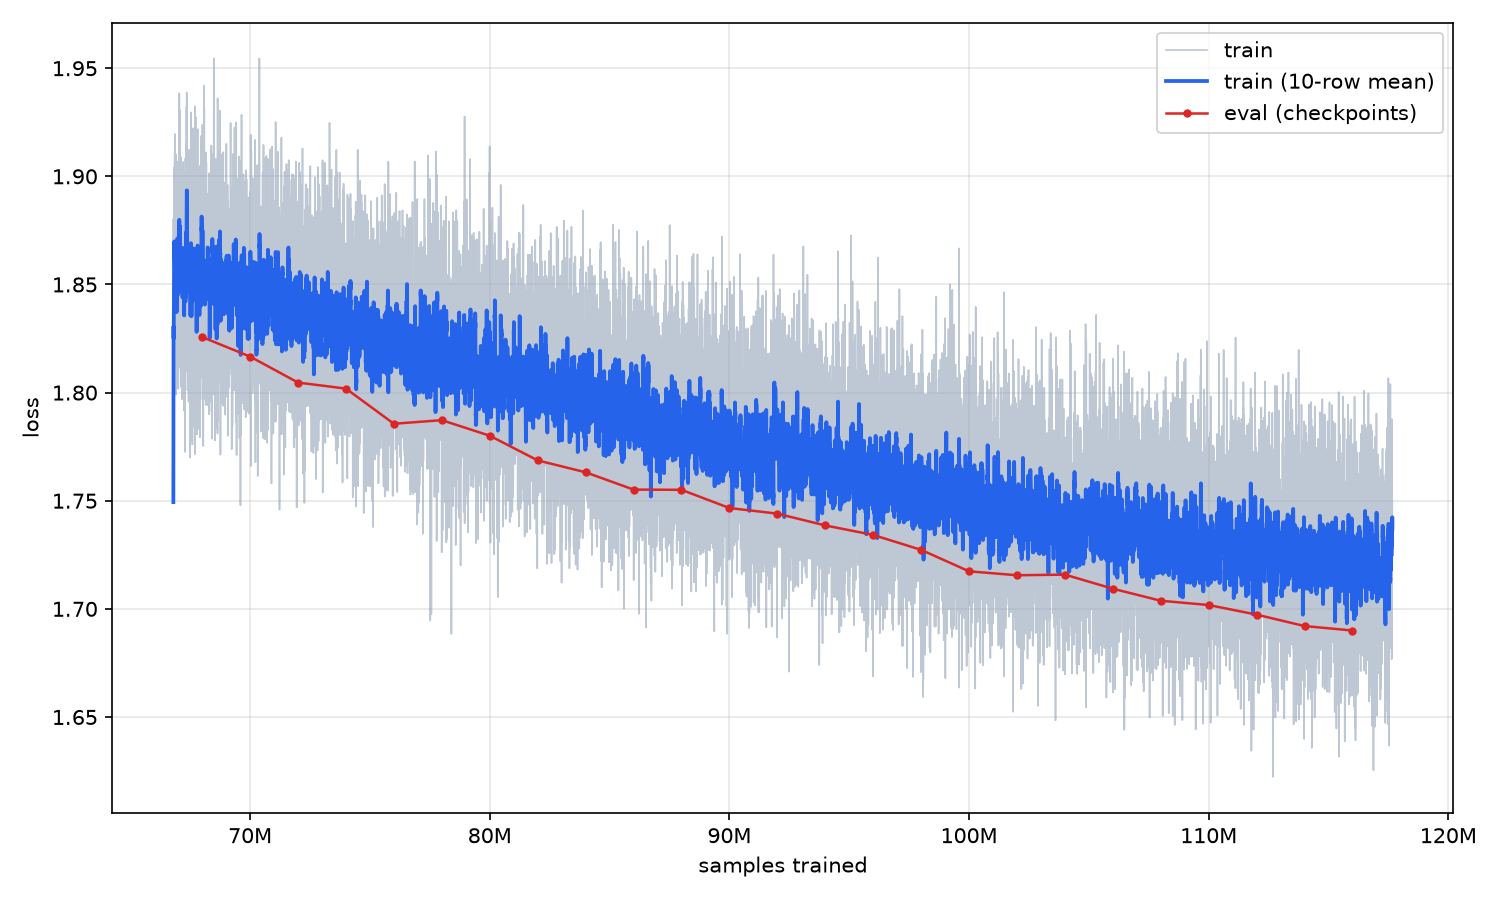
\includegraphics[width=0.66\textwidth]{loss_curve.png}
\caption{Training and evaluation loss vs.\ cumulative samples trained
(\code{checkpoints/loss\_history.jsonl}, rendered by \code{plot\_loss.py}:
faint raw train points, a 10-row rolling mean, and eval points at
checkpoint cadence). The discontinuity at $\approx$118.5M samples is the
switch to the next archive chunk: both the training and the evaluation
shards were replaced (Section~\ref{sec:resume}), and the learning-rate
schedule was revised at the same boundary (see below), so the losses on
either side are measured on \emph{different} evaluation sets and are not
directly comparable.}
\label{fig:loss}
\end{figure}

On the first chunk (66.8M--118.5M samples of the retained history), the
eval loss falls from 1.826 to a best of 1.690 nats at 116.3M, still
improving when the chunk ended. At the chunk boundary the recorded eval
loss jumps to 1.796 and settles at $\approx$1.88 (values 1.878--1.901)
on the new chunk's evaluation set, with the recent training mean around
1.90. The lr history confirms it: the first segment follows an earlier
schedule revision (a cosine decay that had reached its
$3\times10^{-5}$ floor by $\approx$110M samples); at the boundary the
current geometric schedule (Section~\ref{sec:train}), keyed to the
cumulative sample count, resumed at $2.65\times10^{-4}$ and decayed to
$2.62\times10^{-4}$ at 127M samples.

Reading the absolute numbers with the primer's yardsticks: the best
first-chunk eval cross-entropy of 1.690 nats corresponds to a
perplexity of $e^{1.690} \approx 5.4$ --- on average, the model behaved
as if choosing uniformly among 5--6 candidate moves, and placed
$e^{-1.690}\approx 18\%$ probability on the move the human actually
played. Uniform guessing among the $\sim$29.7 legal moves of an average
position would cost $\ln 29.7 = 3.39$ nats ($\approx$3.4\%) --- so the
model extracts about 1.7 nats of human predictability from the position
alone. The current chunk's $\approx$1.88 (perplexity $\approx$6.6,
$\approx$15\%) is measured on a different eval set with a schedule
effectively starting a new annealing phase --- two progress reports of
one continuing run, not an A/B comparison.

\subsection{Scope and honesty}

The move-match, cross-Elo and KL reports of Section~\ref{sec:eval} are
implemented and ready (\code{python evaluate.py}), but their numbers are
not re-measured for this snapshot --- the figures above are the loss
artifacts produced so far. The calibrations to keep in mind: 40--55\%
human--human agreement is the practical ceiling for move-match, and a
near-zero KL would brand the Elo-conditioning story a failure regardless
of how good the accuracy looks.

% =====================================================================
\section{Discussion and Limitations}\label{sec:limits}

\paragraph{Five moves of memory.} The model sees exactly the last five
moves. Human strength expresses itself over far longer horizons ---
repetition draws, long-term plans, clock management --- none of which
fit in a 5-token window. The position fields also omit the halfmove
clock, so even a looming threefold repetition is undetectable. Longer
history --- or a learned compressed game state --- is the obvious next
step.

\paragraph{A policy, not a player.} The model is a pure \emph{policy}: it
scores moves but never plans --- no search, no lookahead, no evaluation
of the resulting position beyond what the transformer absorbed during
training. Strength emerges only by imitation, in contrast with
game-playing systems built around search.

\paragraph{Elo as a blunt conditioning signal.} A 100-point bucket is
coarse, and rating summarizes \emph{results}, not style: two 1600
players can have opposite weaknesses. Per-player style modeling, or
conditioning on time control (bullet and classical blunder very
differently --- the archive mixes them), are natural refinements.

\paragraph{Population skew, and moves vs.\ games.} The data is the Lichess
population --- online, fast time controls, self-selected --- and the 90/10
split is temporal within each archive, so evaluation measures
generalization to slightly-later games of the same population, not to
chess at large. And move-level fidelity is not game-level fidelity:
matching the distribution of individual human moves does not guarantee
that sampled \emph{games} look human --- blunder correlation, time-trouble
behavior and strategic consistency are game-level phenomena a per-move
loss never sees.

\paragraph{Related work.} The closest published system is Maia
Chess~\cite{maia}: networks trained by supervised imitation on games
bucketed by rating, with the same goal of human-like strength control.
chess3 differs mainly in its transformer-over-fields tokenization, the
Elo token as a single conditioning input across one model, and the
legal-restricted softmax tied to a fixed output vocabulary.

% =====================================================================
\section{Conclusion}\label{sec:conclusion}

chess3 shows that a compact, readable transformer --- 26M parameters,
74 fixed tokens, one tied embedding --- trained on more than a hundred
million real human move decisions produces a
distribution-over-moves conditioned on requested strength. The
engineering is as much the result as the model: an 80-byte record
format and precomputed CSR legal-move lists that make 119M samples
cheap to iterate over; a per-field tokenization that eliminates id
collisions by construction; a loss that spends all its signal on the
moves that can actually be played; and checkpoint/resume machinery that
lets one model drink from a stream of monthly archives without starting
over. The evaluation suite answers the question the project stands for
--- not ``is it accurate'' but ``is it human, and is it human \emph{at}
the requested rating.'' The loss trajectory so far (3.39 nats of raw
uncertainty reduced to $\approx$1.7--1.9) says the position and history
carry strong, learnable human signal; the cross-Elo and KL probes are
the instruments that will certify the rest.

% =====================================================================
\appendix
\section{Reproducing the Pipeline}\label{sec:repro}

Everything runs from the repository root; the Python scripts use the
project's virtual environment (\code{venv/}) and the dependencies in
\code{requirements.txt}.

\begin{lstlisting}[style=shell, caption={End-to-end commands.}]
# 1. fetch one monthly archive (~1.5 GB, resumable)
python download_lichess_db.py --month 2026-05

# 2. generate the move vocabulary (idempotent, deterministic)
python move_vocab.py

# 3. games -> binary shards; chunk k of the same archive:
#    --skip-games 2000000 * (k - 1)
python process_lichess_db.py --max-games 1000000

# 4. train (interruptible)
python train.py --epochs 1 --device gpu:0

# 5. resume (also after swapping in a fresh data chunk)
python train.py --resume --checkpoint-cadence 1000000

# 6. render the loss curve
python plot_loss.py

# 7. the three evaluation reports
python evaluate.py --samples 50000

# 8. one-position inference
python infer.py --elo 1800 --pgn "1. e4 e5 2. Nf3 *"

# 9. the GUI (board at localhost:3000)
cd gui && npm run dev
\end{lstlisting}

Each Python module also carries a \code{\_self\_test()} runnable with
\code{python <module>.py}: \code{model.py}, for instance, verifies the
record layout, a forward pass, the masked loss and the parameter count.

% =====================================================================
\begingroup
\setlength{\multicolsep}{3pt}
\begin{multicols}{2}
\begin{thebibliography}{9}\footnotesize

\bibitem{attention}
A.~Vaswani, N.~Shazeer, N.~Parmar, J.~Uszkoreit, L.~Jones, A.~Gomez,
L.~Kaiser, and I.~Polosukhin.
\newblock Attention is all you need.
\newblock \emph{Advances in Neural Information Processing Systems}, 2017.

\bibitem{gpt2}
A.~Radford, J.~Wu, R.~Child, D.~Luan, D.~Amodei, and I.~Sutskever.
\newblock Language models are unsupervised multitask learners.
\newblock \emph{OpenAI Technical Report}, 2019.

\bibitem{adamw}
I.~Loshchilov and F.~Hutter.
\newblock Decoupled weight decay regularization.
\newblock \emph{International Conference on Learning Representations}, 2019.

\bibitem{rmsnorm}
B.~Zhang and R.~Sennrich.
\newblock Root mean square layer normalization.
\newblock \emph{Advances in Neural Information Processing Systems}, 2019.

\bibitem{maia}
K.~McIlroy-Young, S.~Sen, J.~Kleinberg, and A.~Anderson.
\newblock Aligning superhuman agents with human behavior: Maia chess.
\newblock \emph{arXiv:2003.07186}, 2020.

\bibitem{lichess}
Lichess.
\newblock Lichess open database: monthly dumps of all rated games.
\newblock \url{https://database.lichess.org}

\end{thebibliography}
\end{multicols}
\endgroup

\end{document}
